\chapter{机器人移动算法建模}
本文中主要以环形空间中最小移动算法为研究对象。本章节主要介绍使用nuXmv对机器人、最小移动算法进行建模。详细描述了在半同步调度策略、完全同步调度策略和完全异步调度策略下,最小移动算法模型之间的差别。使用LTL规格描述最小移动算法的非冲撞性、非互换性和非终止性。

\section{机器人建模} 
利用nuXmv提供的参数化模块(parameterized module)对机器人进行建模。在机器人模型中使用状态变量分别定义空间位置、移动阶段、移动策略和调度策略。上述这些都是机器人模型的基本属性。

\subsection{空间位置变量}
环形空间探索是多自主机器人协作任务,机器人只能通过空间环境快照,匹配移动算法,完成移动决策。在机器人模型中,可以将每个机器人的所在的空间位置设置成公共变量。这样在实例化机器人时,传入空间中所有机器人的位置变量,这样机器人可以通过传入的机器人位置计算出空间环境快照。

\vspace{0.5cm}

\begin{bfseries} 定义1 \quad 空间位置变量 \quad \end{bfseries} 环形空间中有k个机器人,其所在探索空间中位置的编号使用符号$c_{\left(r\right)}$,$c_{\left(r\right)} \in Pos$。

\vspace{0.5cm}


\subsection{移动阶段变量}


\subsection{移动策略变量}


\subsection{调度策略变量}


\section{环境快照建模}

\section{移动算法建模}

\section{永恒探索建模}

\section{调度策略建模}

\subsection{半同步调度策略建模}

\subsection{完全同步调度策略建模}

\subsection{完全异步调度策略建模}

\section{本章小结}






\begin{lstlisting}
MODULE robot(p1,p2,...)
     VAR
         phase : {lc,m};
         move : -1..1;
         dispatcher:{choose,steady};
     ...
\end{lstlisting}

上述声明的是机器人模块,模块名称为robot,并且模块带有位置环形空间所有机器人位置传入参数p1,p2,...。 在机器人模块实例化时,参数列表第一个位置值\verb|p1|赋值为当前实例机器人在环形空间中的位置值,以当前机器人位置为起点,沿着环形空间顺时针方向依次是p2、p3...,即参数列表是以当前实例机器人的位置为起点,沿着环形空间顺时针方向上的机器人依次传入。

机器人的移动算法是机器人在计算操作时,作为移动决策的判断依据。在nuXmv建模过程采用顺时针或者逆时针相邻两个机器人的之间的没有机器人空间位置结点的个数作为匹配依据。相邻机器人A到机器人B之间没有机器人空间位置结点个数使用$gap_{A \rightarrow B}^F$表示,其中$F \in \left\{+,-\right\}$表示\verb|gap|的计算取值方向,\verb|+| 表示顺时针,\verb|-| 表示逆时针。

$gap_{A \rightarrow B}^F$的计算公式如下:

$$gap_{A \rightarrow B}^+ = \left(c \left( B \right) - c \left( A \right) + n\right) \;  mod \; n $$

$$gap_{A \rightarrow B}^- = \left(n - \left( \left( c \left( B \right) -  c \left( A \right) +n\right) \; mod \; n \right) \right) \; mod \; n $$

\begin{figure}[!hbt]
	\centering
	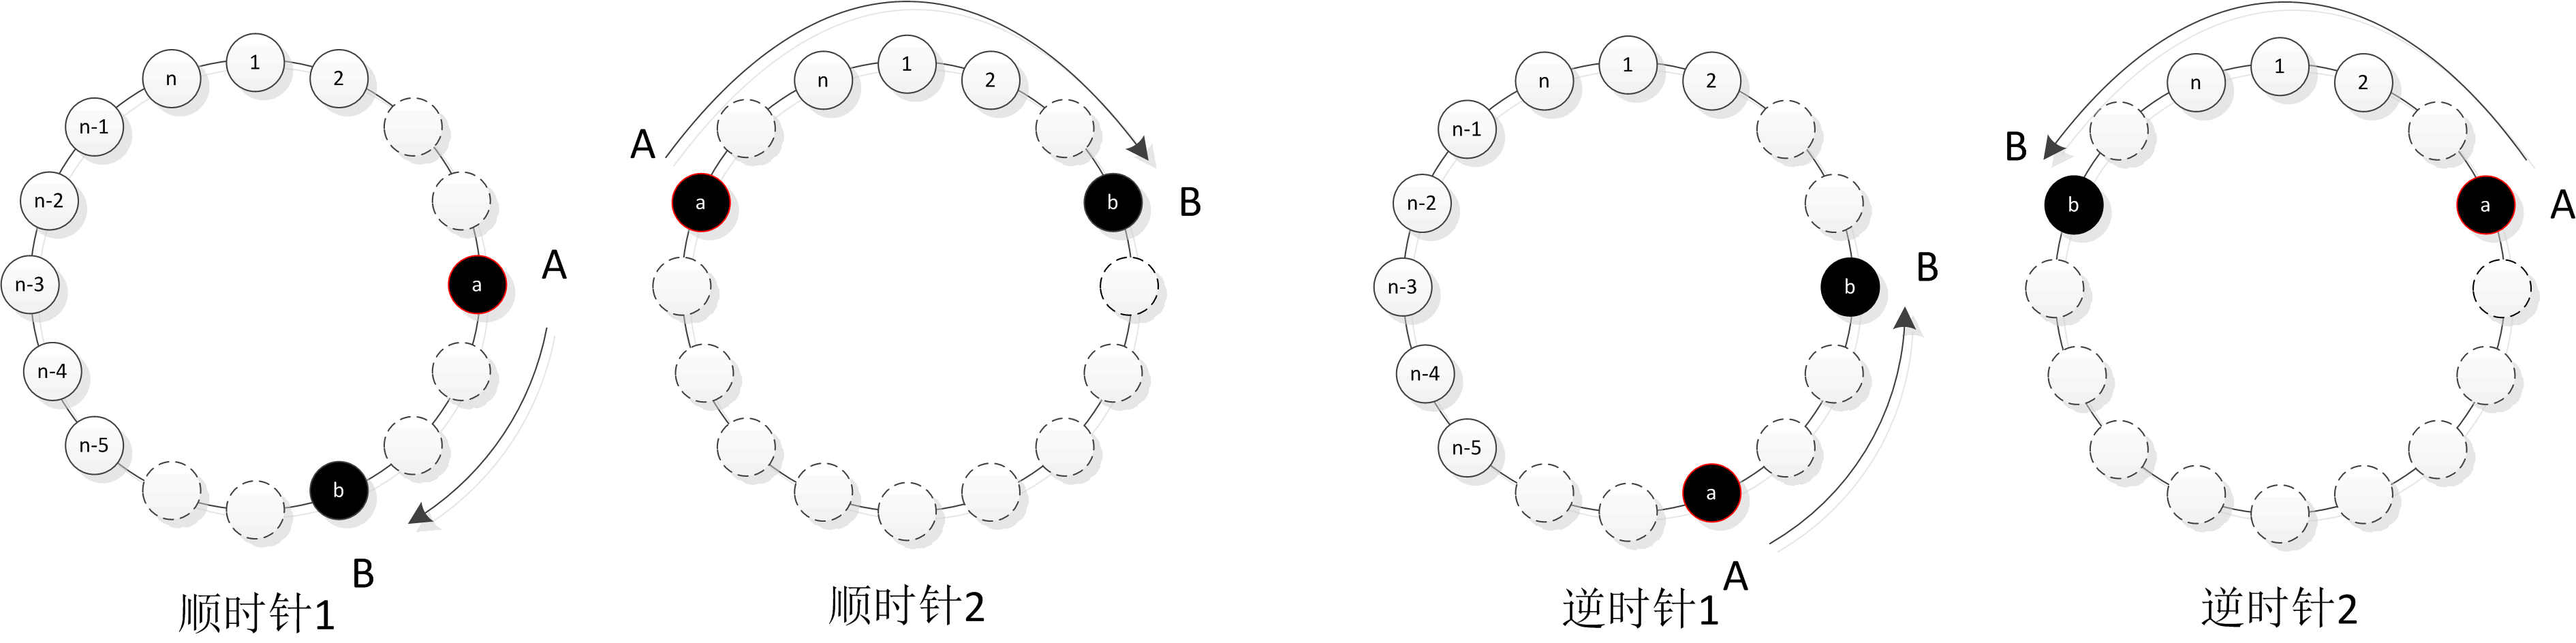
\includegraphics[width=6 in]{fig/gap.png}
	\caption{机器人A和B之间顺时针和逆时针gap计算示意图}
	\label{fig:gap}
\end{figure}

计算公式中n表示环形空间位置结点个数。机器人在环形空间中任意一个时刻都有占据一个空间位置。如图\ref{fig:gap}中所示,环形空间结点的位置是从数字0开始验证环形空间顺时针方向依次递增编号,最后一个编号为n-1,其中n是表示环形空间中位置结点的个数。图中顺时针1和顺时针2、逆时针1和逆时针2 可以看出,当顺时针和逆时针计算机器人A到机器人B的$gap_{A \rightarrow B}^F$ 时,机器人A和机器人B 之间包含位置结点为0 的情况。机器人B与机器人A之间的顺时针间隔为两者节点位置的差加n再以n为基数取模。逆时针的间隔则为n减去顺时针的间隔得到的结果再以n为基数取模.之所以继续取模是考虑A与B 位置重叠的情况,此时,顺时针与逆时针方向的间隔均为0。

假设机器人r的快照F-R视觉快照$\delta_{c\left( r \right)}^F$满足移动算法中的某条规则L,记为$match\left(\delta_{c\left( r \right)}^F,L\right)$。其中规则L可确定的移动方向使用符号$\beta_{\left(L\right)}$ 表示。机器人在每次计算阶段之后,会获取一个移动决策前进(Front),后退(Back) 或者保持不动(Idle),那么分别对应的移动量为1,-1,0。所以机器人r的移动决策可以使用其移动量$M_{\left(r\right)}$表示,具体计算公式如下:

$$ M_{\left(r\right)} = \left\{
\begin{array}{lcl}
1 \quad \, if \left( match \left( \delta_{c\left(r\right)}^F,L\right) \land F=+ \land \beta\left(L\right) = Front\right) \lor \\ \quad \quad  \left(match \left( \delta_{c\left(r\right)}^F,L\right) \land F=- \land \beta\left(L\right) = Back \right) \\
-1 \quad if \left( match \left( \delta_{c\left(r\right)}^F,L\right) \land F=- \land \beta\left(L\right) = Front\right) \lor \\ \quad \quad  \left(match \left( \delta_{c\left(r\right)}^F,L\right) \land F=+ \land \beta\left(L\right) = Back \right) \\
0 \quad \quad  otherwise
\end{array}
\right. $$

对于环形空间,若机器人\verb|r|在空间位置$c\left(r\right)$的顺时针和逆时针快照相同$\delta_{c\left(r\right)}^+ = c\left(r\right)}^-$,也就是说机器人\verb|r|的快照是对称的。若此时机器人r的快照匹配移动算法中某条规则L,根据规则L 得出的移动方向$\beta\left(L\right)$无论是前进或者后退,即机器人的移动量可以是1或者-1,此时机器人会随机选择其中一个作为最终的移动决策。若\verb|r|的为快照不匹配算法当中的任意一个移动规则时移动量就为$M_{\left(r\right)}=0$。

下面代码描述环形空间的节点数为n=10,机器人个数为k=3时的最小移动算法。$next\left(move\right)$ 是机器人\verb|r|的移动量$M_{\left(r\right)}$。$ phase = lc$ 是移动规则匹配的前置条件,当机器人处于观察计算阶段时,才会匹配移动算法。

\begin{lstlisting}
     next(move) :=          --变量 move 在下一步的值
         case
            phase = lc & ((p2 - p1 + 10) mod 10 = 1) & ((p3 - p2 + 10) mod 10 = 3) :  -1;
            --RC1顺时针
            phase = lc & ((10 - ((p3 - p1 + 10) mod 10)) mod 10 = 1) & ((10 - (p2 - p3 + 10) mod 10) mod 10 = 3) : 1;
            --RC1逆时针
            ...

            phase = lc & ((p2 - p1 + 10) mod 10 >= 1) & (((p2 - p1 + 10) mod 10) = ((p1 - p3 + 10) mod 10)) & ((p3 - p2 + 10) mod 10 != (p2 - p1 + 10) mod 10) :  {1,-1};
            --RC2顺时针
            phase = lc & ((10 - ((p3 - p1 + 10) mod 10)) mod 10 >= 1) & ((10 - ((p3 - p1 + 10) mod 10)) mod 10 = (10 - ((p1 - p2 + 10) mod 10)) mod 10) & ((10 - (p2 - p3 + 10) mod 10) mod 10 != (10 - ((p3 - p1 + 10) mod 10)) mod 10) :  {1,-1};
            --RC2顺时针

            ...

            TRUE  :   0;
            --other
         esac;
\end{lstlisting}

代码3-4行描述规则RC1的顺时针方向的匹配,p1表示当前机器人实例的自身位置,在 p1 位置上的机器人 r 从自身开始,按照顺时针方向,依次计算 p1 到 p2、p2 到 p3 之间的间隔个数.对应匹配RL1中机器人的之间的间隔个数,以此作为机器人 r 顺时针匹配移动算法的依据,当满足匹配时\verb|next(move)|的取值为-1。代码5-6行描述RC1的逆时针方向的匹配,逆时针方向的匹配则是计算 p1 到 p3、p3 到 p2 之间的间隔个数作为匹配依据,当满足匹配时\verb|next(move)| 的取值为1。代码9-12行描述规则RC2的顺时针和逆时针匹配,由于RC2规则描述的是对称情况下的移动规则,对于匹配该规则机器人的移动量可能是-1或者1。

\subsection{机器人移动}
机器人经过观察计算阶段之后,会进入移动阶段。机器人在观察计算和移动两种阶段之间切换。

\begin{lstlisting}
 next(phase) :=
         case
            phase = lc     :  m;
            phase = m      :  lc;
            TRUE           :  phase;
         esac;
\end{lstlisting}

在nuXmv建模过程中,机器人移动阶段状态分为两个:观察计算,符号lc表示;移动,符号m表示。下一个移动阶段状态\verb|next(phase)|取决于当前移动阶段状态phase:当当前阶段状态phase为lc下一个移动阶段状态\verb|next(phase)| 的值为m; 当当前阶段状态phase为m,下一个移动阶段状态\verb|next(phase)|的值为观察计算阶段lc;

当机器人移动阶段状态为移动m时,其下一个位置结点编号为$next\left(c\left(r\right)\right)=c\left(r\right)$。机器人移动至新的空间位置上,改变了整个空间中位置快照,所有机器人会根据新的位置快照,做出对应的移动决策。

\begin{lstlisting}
next(p1) :=
         case
            phase = m & (move + p1) < 0                       : 10 + (move + p1);
            phase = m & (move + p1) >= 0 & (move + p1) < 10   : (move + p1);
            phase = m & (move + p1) >= 10                      : (move + p1) - 10;
            TRUE                                              : p1;
         esac;
\end{lstlisting}

\verb|next(p1)|表示当前模块实例化的机器人下一个位置,这个过程只在机器人当前移动阶段状态phase 为m时才会进行。考虑到空间位置范围问题,当机器人顺时针和逆时针通过位置为0的结点时,都会对新的空间位置值进行对应的调整。将机器人的新的位置计算过程归纳如下:

$$ next\left(p1\right) = \left\{
\begin{array}{lcl}
\left(move + p1\right) + n \quad \quad  if \left(move + p1\right) < 0  \\
\left(move + p1\right)     \quad \quad \quad  if \left(move + p1\right) >= 0 \land \left(move + p1\right) < n \\
\left(move + p1\right) - n \quad \quad  if \left(move + p1\right) >= n
\end{array}
\right. $$



\section{调度策略建模}
nuXmv模块化建模的优点是代码可移植性强,在完全同步调度策略、半同步调度策略和完全异步调度策略进行建模时,主模块和机器人模块的建模代码可以复用。三种不同的调度策略情况下,只需根据不同的调度特有性质进行建模调整。

\paragraph{半同步调度策略建模}
对于半同步调度策略,每个机器人在调度过程中只有选中和非选中两种情况。在机器人模型中定义调度变量\verb|dispatcher|,变量声明如下:

\begin{lstlisting}
 VAR dispatcher : {choose,steady};
\end{lstlisting}

使用关键字\verb|VAR|定义符号枚举类型变量\verb|dispatcher|,表示机器人的调度标识。其枚举元素有\verb|choose|和\verb|steady|,分别表示机器人被选中和没被选中。在半同步调度模型中,机器人的每个移动过程中,是随机调度的。机器人随机调度建模如下:

\begin{lstlisting}
next(dispatcher) :=
         case
            TRUE           :  {choose,steady};
         esac;
\end{lstlisting}

建模代码中机器人下一个调度标识只有一个永真的条件分支,并且取值是\verb|{choose,steady}|,即机器人每次移动过程中下一个调度标识是\verb|choose|和\verb|steady|当中随机取值。机器人在匹配移动算法时,若dispatcher为choose,才进行移动算法的匹配。

\begin{lstlisting}
     next(move) :=          --变量 move 在下一步的值
         case
             dispatcher = choose & phase = lc & ((p2 - p1 + 10) mod 10 = 1) & ((p3 - p2 + 10) mod 10 = 3) :  -1;
            --RC1顺时针
             dispatcher = choose & phase = lc & ((10 - ((p3 - p1 + 10) mod 10)) mod 10 = 1) & ((10 - (p2 - p3 + 10) mod 10) mod 10 = 3) : 1;
            --RC1逆时针

            ...

            TRUE  :   0;
         esac;
\end{lstlisting}

移动算法建模中,对每个移动规则匹配添加先决条件\verb|dispatcher = choose|,表明机器人只有在选中是才会计算移动量,否则移动量永远为0。

\paragraph{完全同步调度策略建模}
完全同步调度策略是半同步调度策略的一种特殊情况,空间中所有机器人在每次移动过程中都会被调度。在半同步调度策略建模的基础上,调整模型中调度标识的值永远是选中\verb|choose|:

\begin{lstlisting}
next(dispatcher) :=
         case
            TRUE           :  choose;
         esac;
\end{lstlisting}

\paragraph{完全异步调度策略建模}
完全异步调度策略中所有机器人的移动都是并行的,在nuXmv中实例化机器人模型时,通过关键字\verb|process|声明实例是异步的。

\begin{lstlisting}
VAR
     r1 : process robot(pos1,pos2,pos3);
     r2 : process robot(pos2,pos3,pos1);
     r3 : process robot(pos3,pos1,pos2);
\end{lstlisting}

实例化三个异步机器人r1、r2、r3,在模型验证的过程中,为了确保机器人公平获得执行时间片,可以在机器人模块定义中添加公平性约束。

\begin{lstlisting}
  FAIRNESS
       running
\end{lstlisting}


\section{永恒探索性质}
判定移动算法是否是永恒探索算法,需要移动算法满足三条性质:非冲撞性、非互换性和非终止性。下面以环形空间位置数为10,机器人数为3的最小移动算法为例,任意机器人在任意初始位置,使用LTL公式描述永恒探索算法的三条性质并验证模型对性质的满足性。主模块中声明三个机器人位置变量pos1、pos2、pos3,作为全局变量记录三个机器人的位置。建模时设定三个机器人位置排列顺序是按照顺时针方向依次排列pos1、pos2、pos3。

\begin{lstlisting}
MODULE main
   VAR
     pos1 : 0..9;
     pos2 : 0..9;
     pos3 : 0..9;
     r1 : robot(pos1,pos2,pos3);
     r2 : robot(pos2,pos3,pos1);
     r3 : robot(pos3,pos1,pos2);
\end{lstlisting}

环形空间结点数为n时,空间位置结点编号为0...n-1。当n=10时,机器人的位置编号范围是0到9。在机器人模块实例化时,传入参数列表的第一个参数为当前机器人实例的位置值,后续依次是顺时针方向上机器人位置。例如机器人r1实例化中,第一位参数pos1,表示当前实例是pos1位置上的机器人,并且后续是以pos1为起点顺时针方向依次是pos2和pos3,进行位置参数传入。

使用LTL定义机器人初始位置时,只需限制每个机器人位置的范围和顺时针排列次序。

\begin{lstlisting}
(((pos3 > pos2) & (pos2 > pos1)) | ((pos1 > pos3) & (pos3 > pos2)) | ((pos2 > pos1) & (pos1 > pos3)))
\end{lstlisting}

按照顺时针方向,pos1、pos2、pos3的大小次序有三种可能性:1、pos1<pos2<pos3;2、pos2<pos3<pos1;3、pos3<pos1<pos2;在nuXmv中未给变量分配初始值时,会对该变量的所有取值可能性进行穷举验证。该初始化定义可以实现机器人初始位置任意性的描述。

\paragraph{非冲撞性}
非冲撞性是指离散空间模型中,同一时刻同一位置结点上至多只有一个机器人,使用LTL描述就是同一时刻任意两个机器人所在位置不能相同,如下:

\begin{lstlisting}
LTLSPEC  (((pos3 > pos2) & (pos2 > pos1)) | ((pos1 > pos3) & (pos3 > pos2)) | ((pos2 > pos1) & (pos1 > pos3)))  ->  (G ((pos1 != pos2) & (pos2 != pos3) & (pos1 != pos3)))
\end{lstlisting}

上述LTL定义中,三个机器人位置pos1、pos2和pos3的初始化位置是任意的。nuXmv中LTL符号G表示在将来所有时刻都满足一定条件,在非冲撞性中,表示将来所有时刻都满足pos1、pos2和pos3中任意两个位置都不都相同。

\paragraph{非互换性}
非互换性是指非互换性对应的LTL公式表示如果两个机器人$r_i$与$r_j$物理上相邻,即其所在节点的编号相差1,则一定不会出现$r_i$ 与$r_j$ 在下一个状态位置互换的情况。

\begin{lstlisting}
LTLSPEC  (((pos3 > pos2) & (pos2 > pos1)) | ((pos1 > pos3) & (pos3 > pos2)) | ((pos2 > pos1) & (pos1 > pos3))) -> G ((((pos1 + 1) mod 10) = pos2) -> (X (((pos2+1) mod 10) != pos1)) & (((pos2 + 1) mod 10) = pos3) -> (X (((pos3+1) mod 10) != pos2)) & (((pos3 + 1) mod 10) = pos1) -> (X (((pos1+1) mod 10) != pos3)))
\end{lstlisting}

非互换性中机器人初始位置定义与非冲撞性中的相同。nuXmv中LTL符号X表示在下一个时刻都满足一定条件。由于先决条件是机器人位置pos1、pos2和pos3是在环形空间中是顺时针方向获取的,若当前机器人位置加上1后取模等于前面的机器人位置,那么说明它们相邻,在下一个时刻前面的机器人位置加上1后取模等于前面的机器人位置,表明两者交换了位置。例如((pos1 + 1) mod 10)等于前面位置上的机器人位置pos2,表示pos1与pos2相邻,下一个时刻pos2+1取模不能等于pos1,即pos1和pos2位置不能互换。

\paragraph{非终止性}
非终止性离散空间中每个机器人对每个空间位置结点进行反复的巡查。

\begin{lstlisting}
LTLSPEC   (((pos3 > pos2) & (pos2 > pos1)) | ((pos1 > pos3) & (pos3 > pos2)) | ((pos2 > pos1) & (pos1 > pos3))) -> (((G F (pos1 = 0)) & (G F (pos1 = 1)) &...& (G F (pos1 = 9))) & ((G F (pos2 = 0)) & (G F (pos2 = 1)) &...& (G F (pos2 = 9))) & ((G F (pos2 = 0)) & (G F (pos2 = 1)) &...& (G F (pos2 = 9))))
\end{lstlisting}

命题p描述机器人的位置取值,例如pos1=1,pos1=2等等。LTL公式G F p等价于G (F p),F p表示将来的某个时刻p为真,G (F p)表示将来(F p)一直为真,即p在未来的某些时刻为真。在此表示机器人对某个空间结点反复巡查。

\section{本章小结}
本章以最小移动算法为例,详细介绍了使用nuXmv对机器人模块定义包括移动算法建模、移动算法的匹配。根据三种不同调度策略的性质,对建模做了对应调整。使用LTL公式描述永恒探索算法的三条性质:非冲撞性、非互换性和非终止性。通过模型真实的模拟了环形空间中机器人的移动行为,定义了永恒探索算法的性质。

